\documentclass[12pt]{article}

\usepackage{sbc-template}
\usepackage{graphicx,url}
\usepackage[utf8]{inputenc}
\usepackage[T1]{fontenc}
\usepackage[brazilian]{babel}
\usepackage{xcolor}
\usepackage{amsmath}

% ---------------------------------------------------------------
% \pend{...}: trecho que depende dos SEUS dados -> preencher.
% \val{nome}: número gerado por bench/analyze.py (resultados.tex).
% Antes de entregar, busque por "PREENCHER" e não deixe nenhum.
% ---------------------------------------------------------------
\newcommand{\pend}[1]{\ifmmode\text{\textcolor{red}{[PREENCHER: #1]}}\else\textcolor{red}{[PREENCHER: #1]}\fi}
\newcommand{\val}[1]{\ifcsname #1\endcsname\csname #1\endcsname\else\pend{#1}\fi}
\IfFileExists{resultados.tex}{% gerado por bench/analyze.py — não editar à mão
\newcommand{\branchRatioHost}{10{,}03}
\newcommand{\branchRatioVm}{9{,}90}
\newcommand{\dramHost}{84{,}22}
\newcommand{\dramVm}{92{,}83}
\newcommand{\faultHost}{42{,}64}
\newcommand{\faultVm}{92{,}45}
\newcommand{\ijkHost}{1{,}77}
\newcommand{\ijkVm}{1{,}76}
\newcommand{\ikjHost}{18{,}01}
\newcommand{\ikjVm}{17{,}44}
\newcommand{\loneHost}{0{,}70}
\newcommand{\loneVm}{0{,}70}
\newcommand{\nMaxCpuHost}{10}
\newcommand{\nMaxCpuVm}{9}
\newcommand{\nMaxMemHost}{8}
\newcommand{\nMaxMemVm}{8}
\newcommand{\ncpuHost}{10}
\newcommand{\ncpuVm}{10}
\newcommand{\pCpuHost}{0{,}98}
\newcommand{\pCpuVm}{0{,}96}
\newcommand{\pMemHost}{0{,}10}
\newcommand{\pMemVm}{0{,}15}
\newcommand{\peakHost}{21{,}79}
\newcommand{\peakVm}{21{,}76}
\newcommand{\qdoneHost}{14.132}
\newcommand{\qdoneVm}{420.243}
\newcommand{\qdttHost}{137.185}
\newcommand{\qdttVm}{421.770}
\newcommand{\ridgeHost}{0{,}19}
\newcommand{\ridgeVm}{0{,}20}
\newcommand{\sortedHost}{0{,}23}
\newcommand{\sortedVm}{0{,}23}
\newcommand{\speedupMaxCpuHost}{8{,}32}
\newcommand{\speedupMaxCpuVm}{7{,}79}
\newcommand{\speedupMaxMemHost}{1{,}12}
\newcommand{\speedupMaxMemVm}{1{,}17}
\newcommand{\triadHost}{114{,}16}
\newcommand{\triadVm}{111{,}33}
\newcommand{\unsortedHost}{2{,}31}
\newcommand{\unsortedVm}{2{,}31}
}{}

\sloppy

\title{Quanto custa a camada de virtualização?\\
Perfil de desempenho de um MacBook Air com Apple Silicon\\
em macOS nativo e em uma VM Linux}

\author{Lucca Albuquerque Dangelo\inst{1}}

\address{CESAR School -- Recife, PE -- Brasil
  \email{lada@cesar.school}}

\begin{document}

\maketitle

\begin{abstract}
  Linux virtual machines have become the default way to run development tools on
  Apple Silicon laptops, yet the cost of this layer is rarely measured per
  subsystem. This paper characterizes a MacBook Air along six axes (identification,
  CPU/branch prediction, cache hierarchy, virtual memory, storage and parallelism)
  in two environments on the same hardware: native macOS and a Linux VM managed by
  OrbStack. Using portable microbenchmarks, three runs per measurement and median
  reporting, we locate the machine's bottleneck with the roofline model and
  Amdahl's law and quantify where virtualization adds overhead.
  \pend{1 frase com o principal resultado, ex.: ``Compute-bound code showed
  less than X\% overhead, while ...''}
\end{abstract}

\begin{resumo}
  Máquinas virtuais Linux tornaram-se o caminho padrão para usar ferramentas de
  desenvolvimento em notebooks com Apple Silicon, mas o custo dessa camada
  raramente é medido por subsistema. Este artigo caracteriza um MacBook Air em
  seis eixos (identificação, CPU/predição de desvios, hierarquia de cache,
  memória virtual, armazenamento e paralelismo) em dois ambientes sobre o mesmo
  hardware: macOS nativo e uma VM Linux gerenciada pelo OrbStack. Com
  microbenchmarks portáveis, três execuções por medida e relato da mediana,
  localizamos o gargalo da máquina pelo modelo \textit{roofline} e pela Lei de
  Amdahl e quantificamos onde a virtualização acrescenta custo.
  \pend{1 frase com o principal resultado, ex.: ``Código limitado por
  computação teve custo inferior a X\%, enquanto ...''}
\end{resumo}

% =================================================================
\section{Introdução}

Desde a transição da Apple para processadores ARM próprios, a forma mais comum
de usar ferramentas Linux --- compiladores, contêineres, bancos de dados,
ambientes de disciplinas --- em um Mac é executá-las dentro de uma máquina
virtual leve. Ferramentas como OrbStack, Docker Desktop e UTM escondem essa
camada do usuário: o terminal parece local, mas cada instrução, acesso à memória
e operação de disco passa por um hipervisor. A pergunta prática que
estudantes e desenvolvedores raramente fazem é: \emph{quanto isso custa, e
onde?}

A resposta não é um único número. A teoria de virtualização prevê que
instruções comuns de usuário executem diretamente no processador, com custo
próximo de zero~\cite{popek1974,adams2006}; por outro lado, a tradução de
endereços em dois estágios encarece faltas na TLB~\cite{bhargava2008} e a E/S
atravessa camadas adicionais de software~\cite{barham2003,felter2015}. Um custo
pequeno em um eixo pode ser grande em outro, e o gargalo de uma carga de
trabalho depende de onde ela se situa no modelo \emph{roofline}~\cite{williams2009}.

Este trabalho responde, para uma máquina real, à pergunta:
\textbf{onde está o gargalo deste MacBook Air, e quanto dele é imposto pela
camada de virtualização?} Antes de qualquer medição, registramos quatro
hipóteses:

\begin{itemize}
  \item \textbf{H1 (CPU):} código limitado por computação terá custo inferior
    a 5\% na VM, pois roda nativamente com virtualização assistida por hardware.
  \item \textbf{H2 (cache e memória):} os degraus da escada de cache ocorrerão
    nos mesmos tamanhos nos dois ambientes (o hardware é o mesmo), mas a VM terá
    latência maior para conjuntos de trabalho grandes e page faults mais caros,
    devido à tradução de endereços em dois estágios.
  \item \textbf{H3 (disco):} o armazenamento será o eixo de maior custo,
    sobretudo em leituras aleatórias de 4~KiB com fila rasa (QD=1), onde a
    latência de software adicional não é amortizada.
  \item \textbf{H4 (paralelismo):} o \emph{speedup} de código limitado por
    computação crescerá até o número de núcleos de desempenho e se achatará nos
    núcleos de eficiência; código limitado por memória saturará antes, nos dois
    ambientes.
\end{itemize}

As contribuições são: (i) um perfil de desempenho em seis eixos de um MacBook
Air em dois ambientes; (ii) a quantificação do custo da virtualização por
subsistema; e (iii) uma suíte de benchmark aberta e reprodutível, com scripts e
dados brutos\footnote{\pend{link do repositório no GitHub}}.

% =================================================================
\section{Fundamentação e trabalhos relacionados}

\textbf{Virtualização.} Popek e Goldberg~\cite{popek1974} formalizaram as
condições para que uma arquitetura seja virtualizável de forma eficiente: as
instruções sensíveis devem ser privilegiadas, de modo que o hipervisor só
intervenha quando necessário e o restante execute diretamente no hardware.
Adams e Agesen~\cite{adams2006} mostraram que a primeira geração de suporte em
hardware no x86 nem sempre superava a tradução binária em software, justamente
por causa dos custos de transição entre hóspede e hipervisor. O Xen~\cite{barham2003}
reduziu esses custos com paravirtualização, abordagem que sobrevive hoje nos
dispositivos \emph{virtio} usados pelas VMs Linux. Em ARMv8, o processador
oferece um nível de exceção dedicado ao hipervisor (EL2), que o macOS expõe por
meio do \emph{Hypervisor.framework}, usado por ferramentas como o OrbStack.

\textbf{Memória virtual em VMs.} Com tradução em dois estágios (\emph{nested
paging}), uma falta na TLB no hóspede pode exigir percorrer duas tabelas de
páginas aninhadas; Bhargava et al.~\cite{bhargava2008} mostram que esse
\emph{page walk} bidimensional pode multiplicar o número de acessos à memória
em relação ao caso nativo. Por isso, cargas com pouca localidade são as mais
sensíveis à virtualização na hierarquia de memória~\cite{drepper2007}.

\textbf{Comparações empíricas.} Felter et al.~\cite{felter2015} compararam KVM
e contêineres Docker em servidores x86 e observaram custo desprezível para CPU e
memória, mas custo relevante em E/S e rede para a VM. Este trabalho difere em
três pontos: usa uma plataforma ARM de consumo, com núcleos heterogêneos e
memória unificada; compara VM e sistema nativo no mesmo hardware; e organiza a
análise pelos eixos e modelos da disciplina (equação de desempenho, AMAT,
\emph{roofline} e Amdahl)~\cite{hennessy2017,patterson2016,gregg2020}.

\textbf{Modelos de análise.} O modelo \emph{roofline}~\cite{williams2009}
limita o desempenho atingível por $\min(\pi, \beta \cdot I)$, em que $\pi$ é o
pico de computação, $\beta$ a banda de memória e $I$ a intensidade aritmética
(FLOP/byte); o ponto $I^\ast = \pi/\beta$ separa código limitado por memória de
código limitado por computação. A Lei de Amdahl~\cite{amdahl1967} limita o
\emph{speedup} com $N$ núcleos a $S(N) = 1/[(1-p) + p/N]$, em que $p$ é a
fração paralelizável.

% =================================================================
\section{Metodologia}

\subsection{Ambiente}

A Tabela~\ref{tab:amb} descreve os dois ambientes. Ambos rodam sobre o mesmo
hardware, com o notebook ligado à tomada, demais aplicativos fechados e
intervalo entre execuções. Os programas foram compilados com o mesmo compilador
(\texttt{clang}) e as mesmas opções (\texttt{-O2 -pthread}) nos dois ambientes,
para que a diferença medida seja do ambiente e não do compilador.

\begin{table}[ht]
\centering
\caption{Ambientes de teste (dados de \texttt{sysctl} e \texttt{lscpu}).}
\label{tab:amb}
\footnotesize
\begin{tabular}{lll}
\hline
 & \textbf{Host} & \textbf{VM} \\ \hline
Sistema & macOS \pend{versão} & \pend{distro e kernel} \\
Processador & Apple \pend{M?}, \pend{P+E} núcleos & \pend{n.º de vCPUs} \\
Memória & \pend{GB} unificada & \pend{GB alocados} \\
Cache (núcleo P) & L1d \pend{KiB}, L2 \pend{MiB} & (mesmo hardware) \\
Página & \pend{16 KiB} & \pend{4 KiB} \\
Virtualização & -- & OrbStack \pend{versão} (Hypervisor.framework) \\
Compilador & \pend{clang versão} & \pend{clang versão} \\
\hline
\end{tabular}
\end{table}

\subsection{Eixos de medição}

Seguimos os seis eixos do projeto integrador da disciplina, cada um ligado a um
conjunto de aulas e a uma teoria explicativa:

\begin{enumerate}
  \item \textbf{Identificação (A1, A5):} \texttt{sysctl} no macOS e
    \texttt{lscpu} na VM, registrados automaticamente pelo script.
  \item \textbf{CPU e predição de desvios (A5--A7):} soma condicional sobre
    $2^{16}$ inteiros aleatórios, com o vetor desordenado e depois ordenado.
    Uma barreira de compilador dentro do \texttt{if} impede que o desvio seja
    convertido em seleção condicional. Como contadores de hardware
    (\texttt{perf}) não estão disponíveis no macOS nem na VM, o custo da
    predição errada é inferido pela diferença de tempo por elemento.
  \item \textbf{Cache (A8):} \emph{pointer chasing} sobre uma permutação
    cíclica aleatória (algoritmo de Sattolo), com nós de 128~bytes (tamanho da
    linha de cache) e conjuntos de trabalho de 4~KiB a 256~MiB. Cada acesso
    depende do anterior, o que expõe a latência de cada nível.
  \item \textbf{Memória e memória virtual (A9):} tempo do primeiro toque em
    512~MiB recém-mapeados (\emph{page fault} + zeragem), normalizado por KiB
    porque o tamanho de página difere entre os ambientes; banda sustentada pelo
    kernel \emph{triad} do STREAM ($a = b + s\,c$, 24 bytes e 2 FLOP por
    elemento, vetores de 128~MiB).
  \item \textbf{Disco (A11):} \texttt{fio} com \texttt{--direct=1} para
    contornar o cache de páginas: leitura e escrita sequenciais de 1~MiB e
    leitura aleatória de 4~KiB com QD=1 e QD=32, 15~s cada, arquivo de 512~MiB
    no disco nativo de cada ambiente.
  \item \textbf{Paralelismo (A12--A13):} escalonamento forte de 1 a $N$
    threads para dois núcleos: um limitado por computação (32 cadeias
    independentes de FMA em vetores NEON de 2 \texttt{double}) e um limitado por memória (\emph{triad}). A fração
    paralela $p$ é obtida ajustando a Lei de Amdahl por mínimos quadrados.
\end{enumerate}

Para o \emph{roofline}, o teto de computação $\pi$ é o pico do núcleo de FMA em
uma thread e o teto de memória $\beta$ é a banda do \emph{triad}. Como
exemplos de ``código real'', posicionamos duas multiplicações de matrizes
$1024 \times 1024$ em \texttt{double}: a ordem ingênua \emph{ijk}, que percorre
$B$ por colunas, e a ordem \emph{ikj}, que percorre todas as matrizes por linhas.

\subsection{Protocolo}

Cada medida foi executada três vezes em cada ambiente, e reportamos a
\textbf{mediana}. As hipóteses da Seção~1 foram registradas antes da primeira
execução. O custo da VM é dado por $t_{VM}/t_{host} - 1$ para métricas de
tempo e por $x_{host}/x_{VM} - 1$ para métricas de vazão; valores positivos
indicam que a VM foi pior. Todo o processo é automatizado por
\texttt{run.sh} (coleta) e \texttt{analyze.py} (medianas, ajuste de Amdahl,
figuras e tabelas).

\subsection{Ameaças à validade}

(i) O macOS gerencia frequência e alocação entre núcleos P e E sem controle do
usuário; a VM herda essas decisões, e o MacBook Air não tem ventoinha, então
execuções longas podem sofrer \emph{throttling} térmico. (ii) Os tamanhos de
página diferem (16~KiB no macOS e \pend{4~KiB} na VM), o que afeta TLB e
\emph{page faults}. (iii) Sem contadores de hardware, IPC e taxa de
\emph{branch-miss} não são medidos diretamente. (iv) O \texttt{fio} no macOS
usa \texttt{F\_NOCACHE} para emular \texttt{O\_DIRECT}, e o disco da VM é um
arquivo-imagem sobre o APFS, então os dois caminhos de E/S não são idênticos ---
o que é justamente parte do custo que se quer medir.

% =================================================================
\section{Resultados parciais}

A Tabela~\ref{tab:res} resume as medianas; as subseções interpretam cada eixo
com a teoria correspondente.

\begin{table}[ht]
\centering
\caption{Medianas de 3 execuções. ``Custo VM'' positivo indica pior na VM.}
\label{tab:res}
\small
\IfFileExists{tabela.tex}{\begin{tabular}{lrrrr}
\hline
\textbf{Métrica} & \textbf{Unid.} & \textbf{macOS} & \textbf{VM Linux} & \textbf{Custo VM} \\ \hline
Latência L1 (32 KiB) & ns & 0{,}70 & 0{,}70 & +0{,}0\% \\
Latência 4 MiB & ns & 6{,}56 & 9{,}41 & +43{,}4\% \\
Latência DRAM (256 MiB) & ns & 84{,}22 & 92{,}83 & +10{,}2\% \\
Laço com desvio, aleatório & ns/elem & 2{,}31 & 2{,}31 & +0{,}2\% \\
Laço com desvio, ordenado & ns/elem & 0{,}23 & 0{,}23 & +1{,}5\% \\
Page fault (1º toque) & ns/KiB & 42{,}64 & 92{,}45 & +116{,}8\% \\
Banda de memória (triad) & GB/s & 114 & 111 & +2{,}5\% \\
Pico FMA, 1 thread & GFLOP/s & 21{,}79 & 21{,}76 & +0{,}1\% \\
Matriz ijk & GFLOP/s & 1{,}77 & 1{,}76 & +0{,}5\% \\
Matriz ikj & GFLOP/s & 18{,}01 & 17{,}44 & +3{,}2\% \\
Disco seq. leitura 1M & MB/s & 6.097 & 24.360 & -75{,}0\% \\
Disco seq. escrita 1M & MB/s & 5.873 & 13.650 & -57{,}0\% \\
Disco aleat. 4K QD1 & IOPS & 14.132 & 420.243 & -96{,}6\% \\
Disco aleat. 4K QD32 & IOPS & 137.185 & 421.770 & -67{,}5\% \\
\hline
\end{tabular}
}{\pend{rodar analyze.py para gerar a tabela}}
\end{table}

\subsection{CPU e predição de desvios}

No host, o laço com dados aleatórios levou \val{unsortedHost}~ns por elemento,
contra \val{sortedHost}~ns com o vetor ordenado --- uma razão de
\val{branchRatioHost}$\times$. Na VM, a razão foi \val{branchRatioVm}$\times$.
Pela equação de desempenho $T = N \times CPI \times T_{ciclo}$, o número de
instruções é o mesmo nos dois casos; a diferença vem do CPI, inflado pelo
esvaziamento do \emph{pipeline} a cada predição errada.
\pend{interpretar: a razão é parecida nos dois ambientes? Se sim, isso
confirma H1: o preditor de desvios é hardware e a VM não interfere.}

\subsection{Hierarquia de cache}

\begin{figure}[ht]
\centering
\IfFileExists{figs/cache.pdf}{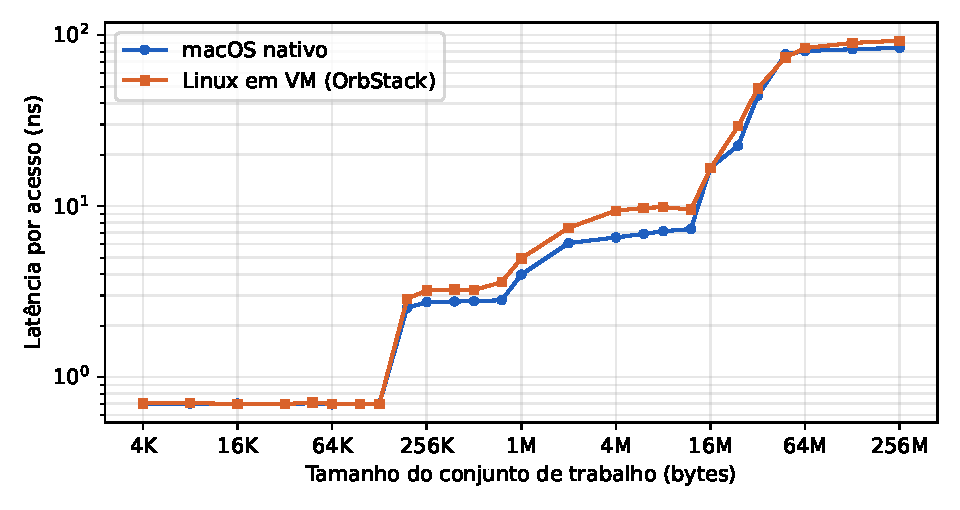
\includegraphics[width=.85\textwidth]{figs/cache.pdf}}{\pend{figs/cache.pdf}}
\caption{Latência por acesso em função do conjunto de trabalho (escala log).}
\label{fig:cache}
\end{figure}

A Figura~\ref{fig:cache} mostra a escada de latência. No host, o acesso
dentro do L1 custou \val{loneHost}~ns e, para 256~MiB (DRAM), \val{dramHost}~ns;
na VM, \val{dramVm}~ns.
\pend{interpretar: (1) os degraus coincidem com o L1d e o L2 da Tabela 1?
(2) a curva da VM se descola da do host só depois de qual tamanho? Isso é
coerente com o custo extra do page walk em dois estágios (H2).}

\subsection{Memória e memória virtual}

O primeiro toque em memória recém-alocada custou \val{faultHost}~ns/KiB no host
e \val{faultVm}~ns/KiB na VM. A banda sustentada (\emph{triad}) foi
\val{triadHost}~GB/s no host e \val{triadVm}~GB/s na VM.
\pend{interpretar: page fault na VM exige saída para o hipervisor na primeira
vez que a página física é usada, então o custo deve ser maior; já a banda
sequencial deve ser parecida, pois depois de mapeada a memória é acessada
diretamente.}

\subsection{Disco}

Na leitura aleatória de 4~KiB, o host atingiu \val{qdoneHost}~IOPS com QD=1 e
\val{qdttHost}~IOPS com QD=32; a VM, \val{qdoneVm} e \val{qdttVm}~IOPS.
\pend{interpretar: com QD=1 cada operação espera a anterior, então a latência
de software da VM pesa inteira; com QD=32 ela é amortizada pelo paralelismo do
SSD. Confirmar ou refutar H3.}

\subsection{Paralelismo e Lei de Amdahl}

\begin{figure}[ht]
\centering
\IfFileExists{figs/scaling.pdf}{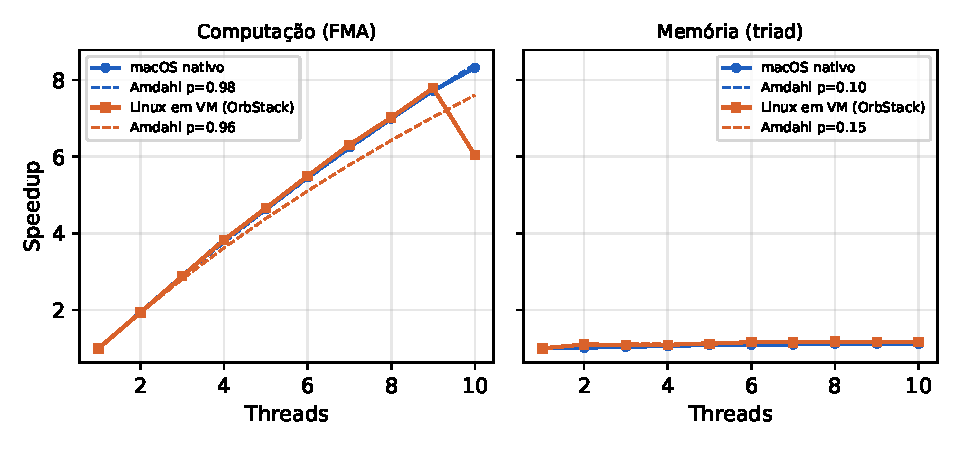
\includegraphics[width=.95\textwidth]{figs/scaling.pdf}}{\pend{figs/scaling.pdf}}
\caption{\emph{Speedup} medido (linha cheia) e ajuste de Amdahl (tracejado).}
\label{fig:scaling}
\end{figure}

No núcleo de computação, o ajuste de Amdahl resultou em
$p = \val{pCpuHost}$ no host e $p = \val{pCpuVm}$ na VM, com \emph{speedup}
máximo de \val{speedupMaxCpuHost}$\times$ e \val{speedupMaxCpuVm}$\times$. No
núcleo de memória, o \emph{speedup} máximo foi \val{speedupMaxMemHost}$\times$
(host) e \val{speedupMaxMemVm}$\times$ (VM).
\pend{interpretar: (1) onde a curva de computação dobra? Deve ser no número de
núcleos P --- os núcleos E são mais lentos, então um p ``baixo'' aqui não é
código serial, é hardware heterogêneo; (2) a curva de memória satura cedo
porque todos os núcleos disputam a mesma banda (memory wall).}

\subsection{\emph{Roofline}: onde está o gargalo}

\begin{figure}[ht]
\centering
\IfFileExists{figs/roofline.pdf}{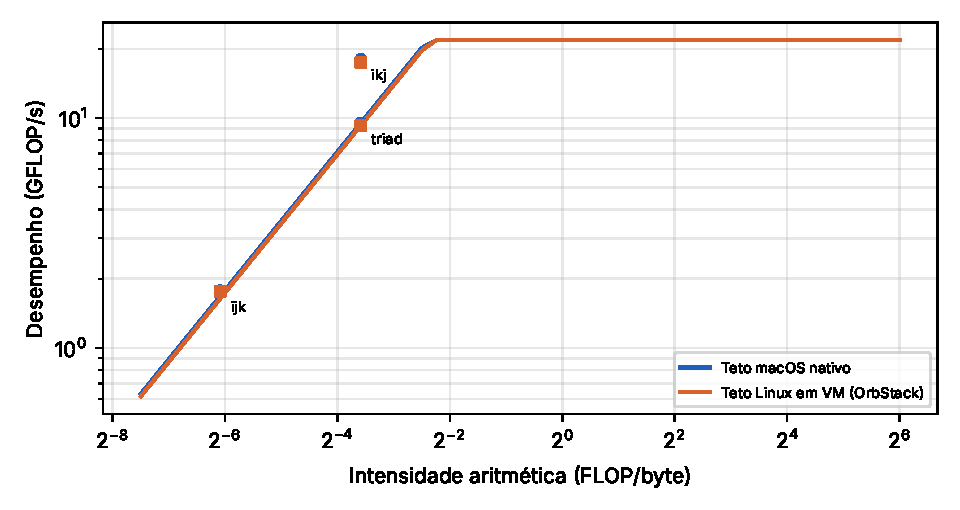
\includegraphics[width=.85\textwidth]{figs/roofline.pdf}}{\pend{figs/roofline.pdf}}
\caption{\emph{Roofline} de uma thread nos dois ambientes.}
\label{fig:roof}
\end{figure}

O pico de computação em uma thread foi \val{peakHost}~GFLOP/s no host e
\val{peakVm}~GFLOP/s na VM. Combinado com a banda do \emph{triad}, o ponto de
inflexão fica em $I^\ast \approx \val{ridgeHost}$~FLOP/byte no host. A
multiplicação \emph{ijk} atingiu \val{ijkHost}~GFLOP/s e a \emph{ikj},
\val{ikjHost}~GFLOP/s --- o mesmo número de operações, com desempenho muito
diferente.
\pend{interpretar: a ijk está bem abaixo da rampa: o gargalo é buscar dados de
B coluna a coluna, sem localidade. A ikj fica acima da rampa da DRAM porque
reaproveita dados no cache, o que eleva sua intensidade aritmética efetiva.
Concluir: o gargalo desta máquina, para código típico, é \_\_\_.}

% =================================================================
\section{Conclusão}

Este artigo caracterizou um MacBook Air com Apple Silicon em seis eixos, em
macOS nativo e em uma VM Linux, para responder onde está o gargalo da máquina
e quanto dele vem da camada de virtualização.
\pend{2--3 frases com a resposta: ``O gargalo desta máquina é \_\_\_, porque
\_\_\_. A virtualização custou menos de \_\_\% em CPU e cache, mas \_\_\% em
\_\_\_.'' Dizer quais hipóteses foram confirmadas e quais foram refutadas.}

Como trabalhos futuros, pretendemos: (i) incluir um hóspede Windows 11 ARM,
para comparar sistemas operacionais sobre o mesmo hipervisor; (ii) medir IPC e
faltas na TLB com contadores de hardware via Instruments; e (iii) comparar VM e
contêiner sobre a mesma VM, repetindo a análise de Felter et al.~\cite{felter2015}
em ARM.

\bibliographystyle{sbc}
\bibliography{refs}

\end{document}
